\documentclass[11pt]{report} 



%-----------------------------------------------------------
\usepackage{subfigure}
\usepackage{vinunicecs}
\usepackage{setspace}
\usepackage[libertine,cmintegrals,cmbraces,vvarbb]{newtxmath}
\usepackage{datetime}

\newdateformat{monthyeardate}{%
  \monthname[\THEMONTH], \THEYEAR}

\renewcommand{\bibname}{REFERENCES}
%-----------------------------------------------------------
% Set your report/thesis particulars 
%-----------------------------------------------------------
%

%\def\RoportType{Capstone project report\xspace} 
\def\RoportType{\xspace}
%\def\RoportType{Project report\xspace}
%
\def\ReportTitle{Title of Your Capstone Project\xspace}
%
\def\Supervisor{Supervisor's Name: yyyy\xspace} 
\def\SupervisorPosition{Assistant Professor XXX\xspace}
%
%\def\reportSubmissionDate{\today}
\def\reportSubmissionDate{\monthyeardate\today}
\def\reportSubmissionTerm{\monthyeardate\today}


%-----------------------------------------------------------
% List the project members
%-----------------------------------------------------------
%
\def\numberOfAuthors{3} % you can change to other numbers 
%
\def\firstAuthor{Ngo Xuan Phong\xspace} 
\def\firstAuthorID{20200461\xspace}
\def\firstAuthorDedication{Dedicated to \\ \textit{abc}}
%
\def\secondAuthor{Second Author\xspace} 
\def\secondAuthorID{243014000\xspace} 
\def\secondAuthorDedication{To my girl  ...\\ \textit{pqr}}
%
\def\thirdAuthor{Third Author\xspace} 
\def\thirdAuthorID{243014000\xspace} 
\def\thirdAuthorDedication{To \\ \textit{xyz} \\ a good soul.}

%-----------------------------------------------------------

\begin{document}

 \baselineskip=18pt plus1pt
 \setcounter{secnumdepth}{3}
 \setcounter{tocdepth}{3}
 \pagenumbering{roman} 
 \frontmatter{\numberOfAuthors}
 \tableofcontents
 \listoffigures
 \listoftables
 \clearpage
 \pagenumbering{arabic}
%-----------------------------------------------------------
% Include Chapters 
%-----------------------------------------------------------
 \chapter{INTRODUCTION}

Chapter 1 should provide a clear statement of the problem posed by the project, and
why the problem is of interest. It should reflect the scenario, if available. The
introduction also needs to present background information so that the reader can
understand the significance of the problem.


\section{Project Background }

\begin{itemize}
\item Provide literature review: With the aim to provide an overview of relevant research, studies, and theories related to the problem or topic addressed in the project.

\item Relevance and Importance: Why the problem is of interest and importance now; Who will use your proposed solution; State the potential impact of your project results.

\item Current State and Limitations: Describe the current situation or existing solutions and their shortcomings.

\item Transition: Conclude by bridging into the project definition and/or objectives.
\end{itemize}

\section{Project Definition}
Define the problem in terms of the technical details and features that the product, service, or process should have. These details are often set by your advisors to make sure the project is challenging and appropriate for a Capstone project. Here's how to break it down:


\subsection{Problem Statement} 
State the problem in a single sentence or a brief paragraph.


\subsection{Context and Scope}
Define the scope of the problem—what aspects it
encompasses and what it does not cover.


\subsection{Significance and Implications} Explain why solving this problem is important.
What are the potential consequences of not addressing it?


\subsection{Quantification (if any)}
If possible, quantify the problem to demonstrate its magnitude. This could involve presenting relevant statistics, data, or trends.\\


\noindent Remember to keep the definition of the problem concise, focused, and aligned with the goals of your Capstone project. It should be easy to understand and provide a clear sense of direction for the rest of the proposal.

\section{Project Objectives}
The objectives of a Capstone project outline the specific goals and outcomes you and your team aim to achieve through the project. These objectives guide your team and provide a clear focus. When writing the objectives section, make sure they are \textbf{specific, measurable, achievable, relevant, and time-bound (SMART)}. An example is given
below:
\begin{itemize}
\item \textbf{Objective 1}: [Title]
      \begin{itemize}
        \item State the first objective in clear terms.
        \item Describe what you plan to achieve with this objective.
        \item Make it specific and measurable.
      \end{itemize}
\end{itemize}

\begin{equation}\label{eq:EMC}
E = MC^2
\end{equation}


\section{Project Specifications}
Given the project objectives above, you are asked to provide the detailed technical requirements, features, and characteristics that your project must adhere to in order to meet its objectives. These include technical needs, performance expectations, design elements, functionalities, compatibility, and security measures. Specifications guide the project's development, ensuring it meets its objectives effectively and aligns with established criteria.


\begin{figure}[t]
	\centering
	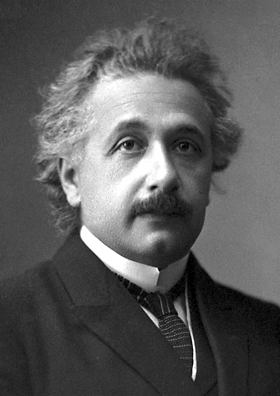
\includegraphics[width=0.5\columnwidth,trim={0cm 0.0cm 0cm 0.0cm}]{Images/Einstein.png}
% 		\vspace{-2pt}
	\caption{\small Albert Einstein is widely regarded as a genius.}
	\label{fig:queue-length}
\end{figure}



\cite{Tsebook05,SamarakoonTWC13,KeyInforcom2007}.
 %-----------------------------------------------------------------
% LaTeX template for a Bachelor Capstone Project Report/Thesis 
% (CSE 499) of the Department of Computer Science and Engineering 
% at the University of Liberal Arts Bangladesh (ULAB)

% Written By: Muhammad Abul Hasan, PhD
% Date Updated: February 08, 2021 (v1.1)
% For any comments or suggestions: muhammad.hasan@ulab.edu.bd
%-----------------------------------------------------------

\chapter{PROJECT MANAGEMENT}

Chapter 2 will assess the ability to work as a team from planning, dividing work,
monitoring progress and making decisions.


%%%%%%%%%%%%%%%%%%%%%%%%%%%%%%%%%%%%%%%%%%%%%%%%%%%%%%
\section{Project Plan}
This plan outlines the project’s timeline, tasks, responsibilities, and milestones. It demonstrates how you've organized and structured the project to achieve its objectives.


%%%%%%%%%%%%%%%%%%%%%%%%%%%%%%%%%%%%%%%%%%%%%%%%%%%%%%
\section{Contribution of Team Members}
\begin{itemize}
\item Highlight the individual contributions of each team member.
\item Discuss how each person's skills, expertise, and responsibilities contribute to the project's success.
\item This section showcases teamwork and collaboration.
\end{itemize}


%%%%%%%%%%%%%%%%%%%%%%%%%%%%%%%%%%%%%%%%%%%%%%%%%%%%%%
\section{Challenges and Decision Making}
Discuss any challenges or unexpected issues that arise during the project. Explain how your team addresses these challenges and how decisions are made. Highlight the decision-making process and how it impacts project outcomes.





 \chapter{SYSTEM DESCRIPTION}
The purpose of the Chapter 3 is to describe the process of designing your project. The detail should be sufficient so that the reader can easily understand what was done. A brief summary of the unique approach your group used to solve the problem should be given, also including a concise introduction to theory or concepts used to analyze and calculate. To improve clarity of presentation, this section may be further divided into subsections as below:

%%%%%%%%%%%%%%%%%%%%%%%%%%%%%%%%%%%%%%%%%%%%%%%%%%%%%%
\section{Block Diagram of the System}
\begin{itemize}
\item Present an overview of the system’s architecture through a block diagram. Each block should represent a key component or module of your project
\item Describe the purpose and functionality of each block, highlighting their
relationships and interactions.
\end{itemize}

%%%%%%%%%%%%%%%%%%%%%%%%%%%%%%%%%%%%%%%%%%%%%%%%%%%%%%
\section{Design of Each Block and Select the Best Alternative}
\begin{itemize}
\item Here, delve into the design details of each individual block from the block diagram. Discuss different design alternatives considered and the rationale behind selecting the final design.
\item If any unique approaches were used, elaborate on them. Explain how each block's design contributes to the overall functionality of the system.
\end{itemize}

%%%%%%%%%%%%%%%%%%%%%%%%%%%%%%%%%%%%%%%%%%%%%%%%%%%%%%
\section{Testing of Each Block}
\begin{itemize}
\item This subsection covers the comprehensive testing procedures conducted for each block.
\item Please note that this subsection can be removed/modified depending on the specific project.
\end{itemize}


%%%%%%%%%%%%%%%%%%%%%%%%%%%%%%%%%%%%%%%%%%%%%%%%%%%%%%
\section{System Implementation}
\begin{itemize}
\item Discuss the practical steps taken to translate the conceptual design into tangible
components. Considerations for scalability, efficiency, and real-world
implementation are detailed.
\end{itemize}

 \chapter{SYSTEM TESTING AND ANALYSIS}


Chapter 4 provides an overview of the implementation and testing phases of the proposed Capstone project. This chapter is dedicated to explaining how the project will be executed, the system will be tested, and the obtained results will be analyzed and discussed in the second semester. The following subsections guide the presentation of this information: 
\begin{itemize}
\item Briefly provide the systematic approach used to conduct system testing (if prototype) amd simulating (if simulation). The testing phase aims to verify the functionality, reliability, and performance of the implemented solution. 
\item Briefly describe the different types of tests performed, including unit testing, integration testing, and user acceptance testing.
\end{itemize}



\begin{table}[!h]
\begin{center}
\begin{tabular}{||c c c c||} 
 \hline
 Col1 & Col2 & Col2 & Col3 \\ [0.5ex] 
 \hline\hline
 1 & 6 & 87837 & 787 \\ 
 \hline
 2 & 7 & 78 & 5415 \\
 \hline
 3 & 545 & 778 & 7507 \\
 \hline
 4 & 545 & 18744 & 7560 \\
 \hline
 5 & 88 & 788 & 6344 \\ [1ex] 
 \hline
\end{tabular}
\caption{\label{demo-table}Your caption.}
\end{center}
\end{table}

 \chapter{CONCLUSION AND RECOMMENDATION}

Chapter 5 should summarize the key findings and outcomes of your Capstone proposal project. This section serves to highlight the achievements, discuss the implications of your work, and offer recommendations for future steps. The following subsections guide the presentation of this information:

%%%%%%%%%%%%%%%%%%%%%%%%%%%%%%%%%%%%%%%%%%%%%%%%%%%%%%
\section{Conclusion}
\begin{itemize}
\item Reiterate the problem addressed, the objectives achieved, and the impact of our proposed solution.
\item By reflecting on the significance of the proposal, you can emphasize the
contributions made to the field and the potential benefits to stakeholders.
\end{itemize}


%%%%%%%%%%%%%%%%%%%%%%%%%%%%%%%%%%%%%%%%%%%%%%%%%%%%%%
\section{Future Recommendation}
\begin{itemize}
\item Provide recommendations for future steps based on your proposal’s outcomes.
\item Identify areas where further refinement, expansion, or exploration will be
warranted. These recommendations provide valuable guidance for subsequent
stages of the project or for other researchers interested in building upon our work.
\end{itemize}

 % Documentation: https://ctan.org/pkg/mitthesis


\addcontentsline{toc}{chapter}{APPENDIX}
\noindent{\bf\huge APPENDIX}  

\lstdefinestyle{mystyle}{
    backgroundcolor=\color{CadetBlue!15!white},   
    commentstyle=\color{Red3},
    numberstyle=\tiny\color{gray},
    stringstyle=\color{Blue3},
    basicstyle=\small\ttfamily,
    breakatwhitespace=false,         
    breaklines=true,                 
    numbers=left,                    
    numbersep=5pt,                  
    showspaces=false,                
    showstringspaces=false,
    showtabs=false,                  
    tabsize=2
}%
\lstset{language=[5.3]Lua,style={mystyle}}%



%-----------------------------------------------------------
\addcontentsline{toc}{chapter}{REFERENCES}
\bibliographystyle{unsrt}
\bibliography{references}
\coverpage{\numberOfAuthors}


\end{document}